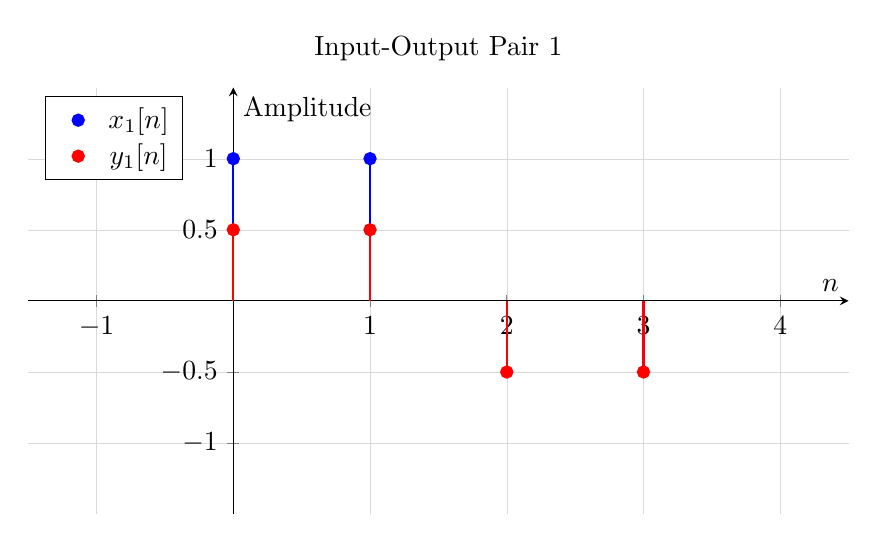
\begin{tikzpicture}
	\begin{axis}[
		width=12cm,
		height=7cm,
		axis lines=middle,
		xlabel={$n$},
		ylabel={Amplitude},
		title={Input-Output Pair 1},
		xmin=-1.5, xmax=4.5,
		ymin=-1.5, ymax=1.5,
		xtick={-1, 0, 1, 2, 3, 4},
		ytick={-1, -0.5, 0.5, 1},
		grid=major,
		grid style={line width=.1pt, draw=gray!30},
		legend style={
			at={(0.02,0.98)},
			anchor=north west,
		}
		]
		
		\addplot[blue, ycomb, thick, mark=*, mark size=2pt]
		coordinates {(0,1) (1,1)};
		\addlegendentry{$x_1[n]$};
		
		\addplot[red, ycomb, thick, mark=*, mark size=2pt]
		coordinates {(0,0.5) (1,0.5) (2,-0.5) (3,-0.5)};
		\addlegendentry{$y_1[n]$};
		
	\end{axis}
\end{tikzpicture}

\vspace{1cm}

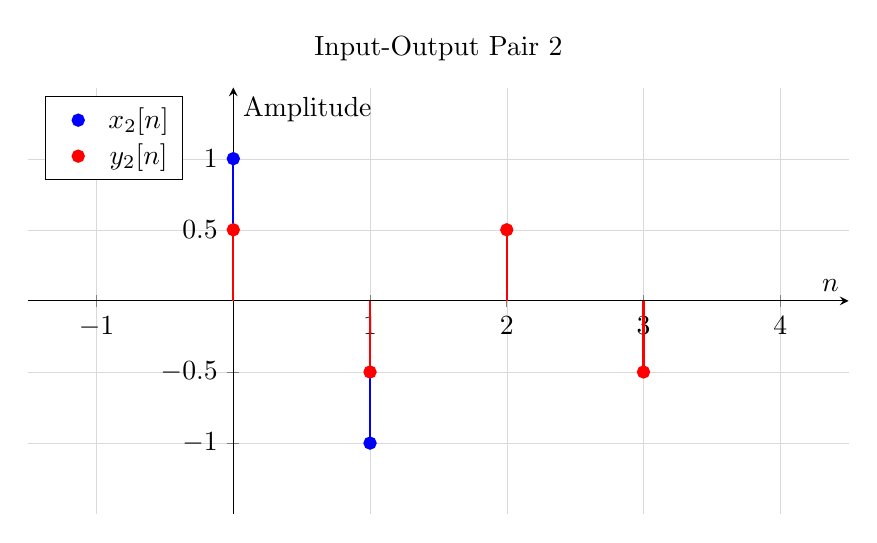
\begin{tikzpicture}
	\begin{axis}[
		width=12cm,
		height=7cm,
		axis lines=middle,
		xlabel={$n$},
		ylabel={Amplitude},
		title={Input-Output Pair 2},
		xmin=-1.5, xmax=4.5,
		ymin=-1.5, ymax=1.5,
		xtick={-1, 0, 1, 2, 3, 4},
		ytick={-1, -0.5, 0.5, 1},
		grid=major,
		grid style={line width=.1pt, draw=gray!30},
		legend style={
			at={(0.02,0.98)},
			anchor=north west,
		}
		]
		
		\addplot[blue, ycomb, thick, mark=*, mark size=2pt]
		coordinates {(0,1) (1,-1)};
		\addlegendentry{$x_2[n]$};
		
		\addplot[red, ycomb, thick, mark=*, mark size=2pt]
		coordinates {(0,0.5) (1,-0.5) (2,0.5) (3,-0.5)};
		\addlegendentry{$y_2[n]$};
		
	\end{axis}
\end{tikzpicture}
